\subsection{Глобальные и локальные модели освещения в компьютерной графике. Модель Фонга.}

\textbf{Глобальные и локальные модели}

Моделировать освещение очень важно, т.к. на основе освещения мы воспринимаем форму объектов. Глаз воспринимает освещение и «реконструирует» трехмерную форму. Моделирование освещения --- ключевой элемент фотореализма.

Полный отраженный свет = сумма вклада от источников света и других поверхностей сцены.

Светоиспускающие источники --- первичные, светоотражающие источники --- вторичные. 
\textbf{Локальные модели} учитывают только первичные источники
света, \textbf{глобальные} --- все источники. 

Поверхность, не освещаемая источником света, все равно может быть видима

Локальные модели при вычислении освещения в данной точке учитывают только положение этой точки относительно первичных источников света.

Существующие модели:
\begin{itemize}
    \item Диффузное отражение (матовый пластик, дерево, бумага) --- модель Ламберта. 
    \item Идеально зеркальное отражение (зеркало) --- модель отражения.
    \item Зеркальное отражение (блики на объекте) --- модели Фонга и Блинна.
\end{itemize}

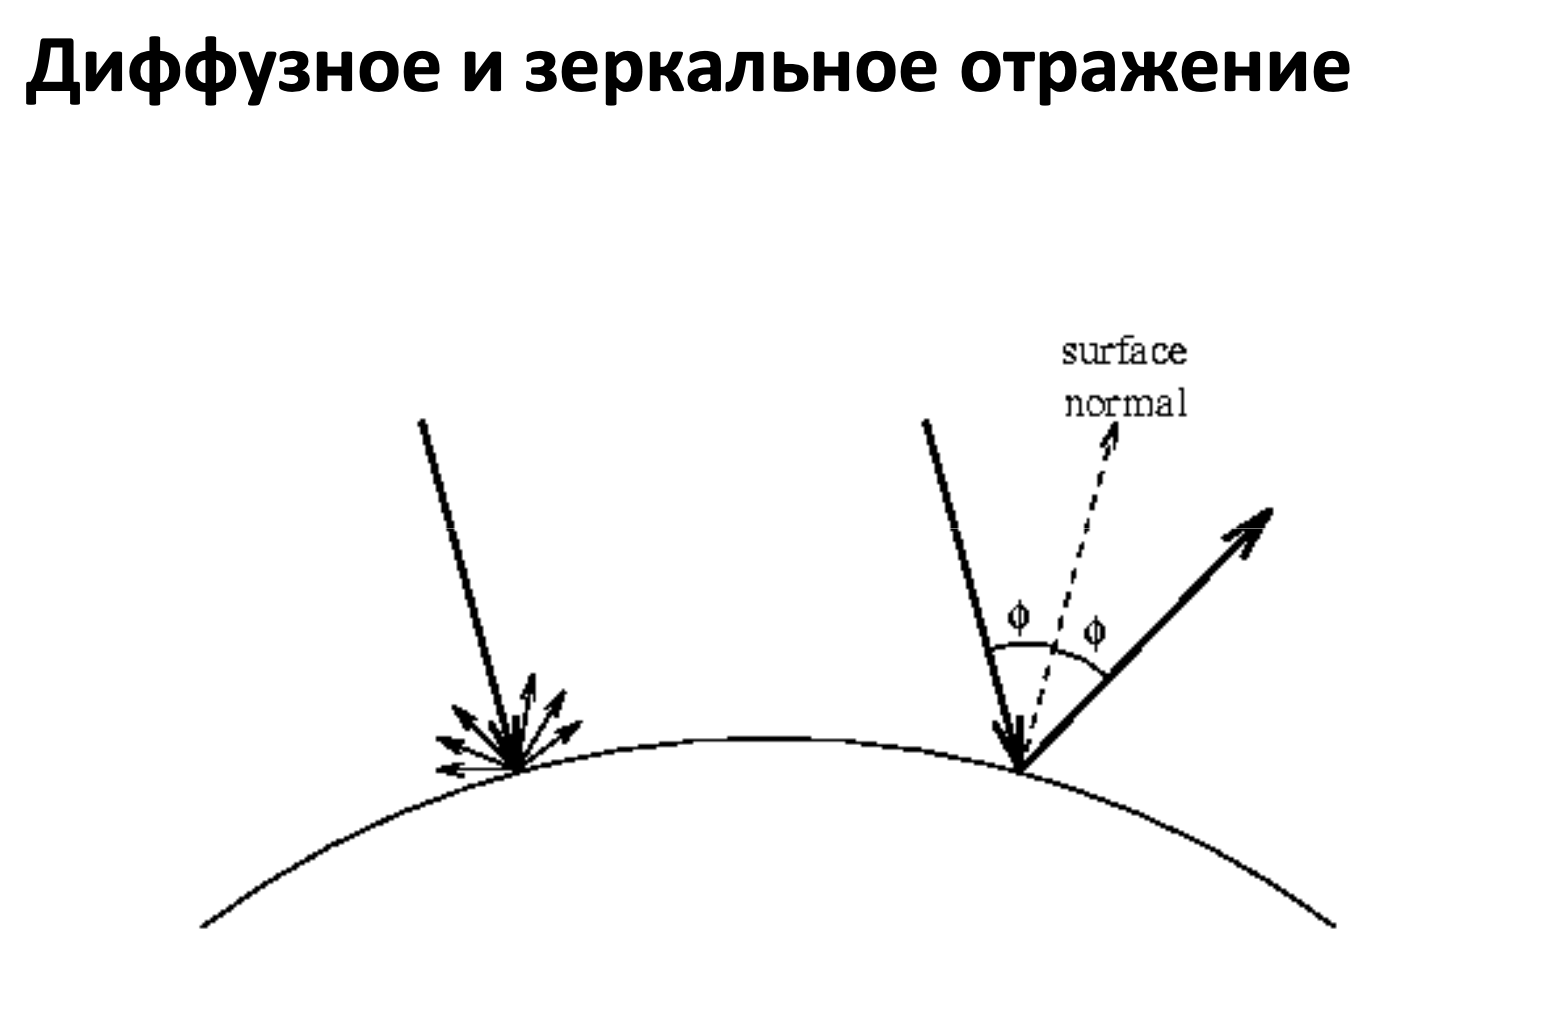
\includegraphics[width=\columnwidth]{pics/reflection.png}

\textbf{Модель Фонга}

Для определения яркости пикселя можно воспользоваться формулой Y=0.3*R+0.59*G+0.11*B.

Расчёт освещения по Фонгу требует вычисления цветовой интенсивности трёх компонент освещения: фоновой (ambient), рассеянной (diffuse) и глянцевых бликов (specular).

\textit{Фоновое освещение} --- это постоянная в каждой точке величина надбавки к освещению. 
Вычисляется фоновая составляющая освещения как: $I_a = a L_a$, где $a$ --- свойство материала воспринимать фоновое освещение (коэффициент фонового освещения), $L_a$ --- мощность фонового освещения.

\textit{Рассеянный свет} при попадании на поверхность рассеивается равномерно во все стороны. 
При расчете такого освещения учитывается только ориентация поверхности (нормаль) и направление на источник света. 
Рассеянная составляющая рассчитывается по закону косинусов (закон Ламберта): $I_d = d \langle S, n \rangle$. 
Здесь $d$ --- свойство материала воспринимать рассеянное освещение (коэффициент рассеянного освещения), $S$ --- направление из точки объекта на источник света, $n$ --- вектор нормали в точке объекта.

\textit{Зеркальный свет} при попадании на поверхность подчиняется следующему закону: <Падающий и отраженный лучи лежат в одной плоскости с нормалью к отражающей поверхности в точке падения, и эта нормаль делит угол между лучами на две равные части>. 
Таким образом отраженная составляющая освещенности в точке зависит от того, насколько близки направления на наблюдателя и отраженного луча: $I_s = k_s \langle r, v \rangle^p$. Здесь $k_s$ --- коэффициент зеркального отражения, $r$ --- направление отраженного луча, $v$ --- направление на наблюдателя, $p$ --- коэффициент блеска, свойство материала.

Итого формула освещения в модели Фонга: $I = I_a + I_d + I_s = a L_a + d \langle S, n \rangle + k_s \langle r, v \rangle^p$.

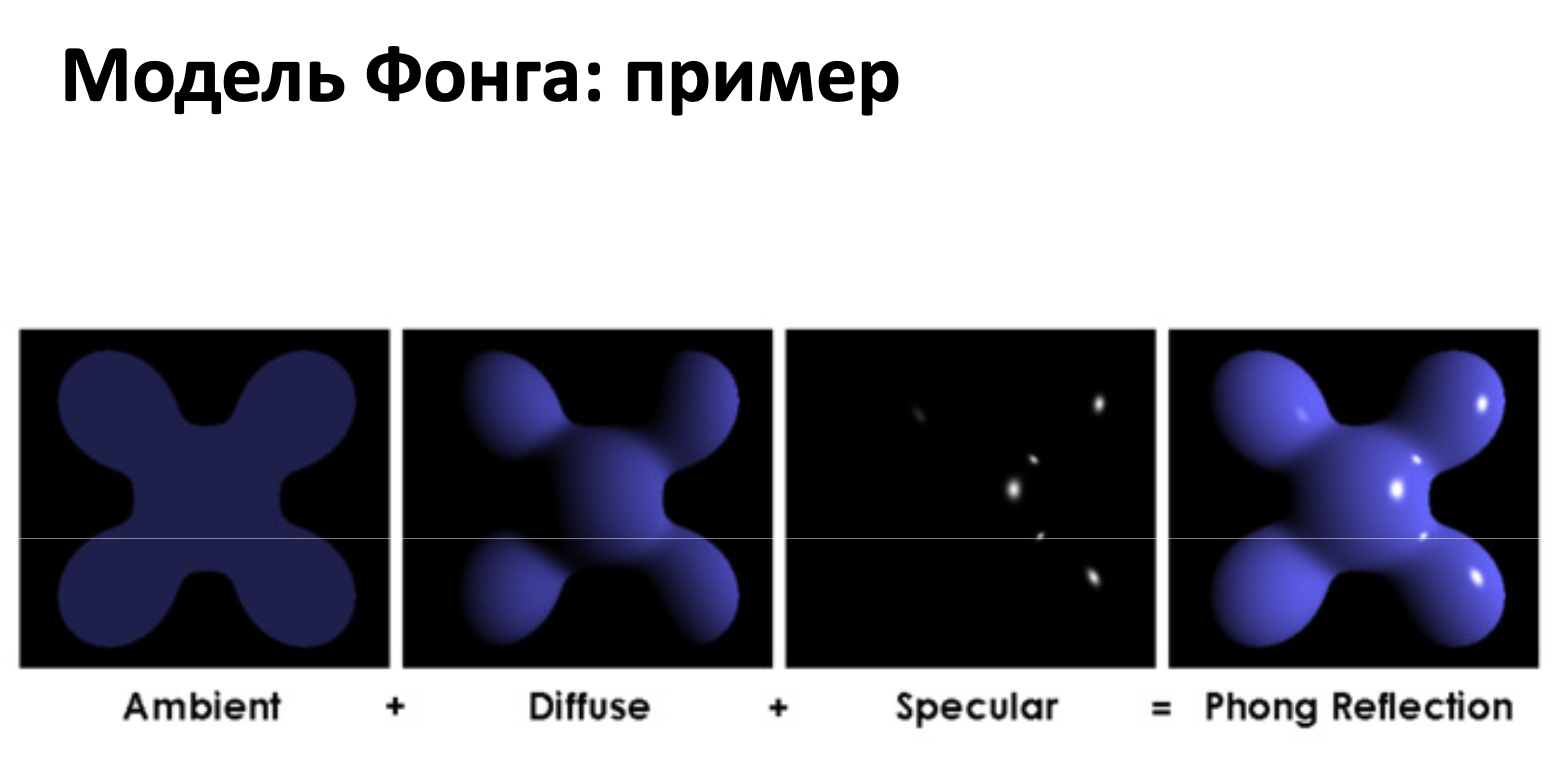
\includegraphics[width=\columnwidth]{pics/fong.png}

% -------- source --------
\bigbreak
[\cite[page 19-26]{iit_graphics}]